% -*- coding: utf-8 -*-
%-------------------------designed by zcf--------------
\documentclass[UTF8,a4paper,10pt]{ctexart}
\usepackage[left=3.17cm, right=3.17cm, top=2.74cm, bottom=2.74cm]{geometry}
\usepackage{amsmath}
\usepackage{graphicx,subfig}
\usepackage{float}
\usepackage{cite}
\usepackage{caption}
\usepackage{enumerate}
\usepackage{booktabs} %表格
\usepackage{multirow}
\newcommand{\tabincell}[2]{\begin{tabular}{@{}#1@{}}#2\end{tabular}}  %表格强制换行
%-------------------------字体设置--------------
\usepackage{times} 
\newcommand{\yihao}{\fontsize{26pt}{36pt}\selectfont}           % 一号, 1.4 倍行距
\newcommand{\erhao}{\fontsize{22pt}{28pt}\selectfont}          % 二号, 1.25倍行距
\newcommand{\xiaoer}{\fontsize{18pt}{18pt}\selectfont}          % 小二, 单倍行距
\newcommand{\sanhao}{\fontsize{16pt}{24pt}\selectfont}  %三号字
\newcommand{\xiaosan}{\fontsize{15pt}{22pt}\selectfont}        % 小三, 1.5倍行距
\newcommand{\sihao}{\fontsize{14pt}{21pt}\selectfont}            % 四号, 1.5 倍行距
\newcommand{\banxiaosi}{\fontsize{13pt}{19.5pt}\selectfont}    % 半小四, 1.5倍行距
\newcommand{\xiaosi}{\fontsize{12pt}{18pt}\selectfont}            % 小四, 1.5倍行距
\newcommand{\dawuhao}{\fontsize{11pt}{11pt}\selectfont}       % 大五号, 单倍行距
\newcommand{\wuhao}{\fontsize{10.5pt}{15.75pt}\selectfont}    % 五号, 单倍行距
%-------------------------章节名----------------
\usepackage{ctexcap} 
\CTEXsetup[name={,、},number={ \chinese{section}}]{section}
\CTEXsetup[name={(,)},number={\chinese{subsection}}]{subsection}
\CTEXsetup[name={,.},number={\arabic{subsubsection}}]{subsubsection}
%-------------------------页眉页脚--------------
\usepackage{fancyhdr}
\pagestyle{fancy}
\lhead{\kaishu \leftmark}
% \chead{}
\rhead{\kaishu 网络安全技术实验报告}%加粗\bfseries 
\lfoot{}
\cfoot{\thepage}
\rfoot{}
\renewcommand{\headrulewidth}{0.1pt}  
\renewcommand{\footrulewidth}{0pt}%去掉横线
\newcommand{\HRule}{\rule{\linewidth}{0.5mm}}%标题横线
\newcommand{\HRulegrossa}{\rule{\linewidth}{1.2mm}}
%-----------------------伪代码------------------
\usepackage{algorithm}  
\usepackage{algorithmicx}  
\usepackage{algpseudocode}  
\floatname{algorithm}{Algorithm}  
\renewcommand{\algorithmicrequire}{\textbf{Input:}}  
\renewcommand{\algorithmicensure}{\textbf{Output:}} 
\usepackage{lipsum}  
\makeatletter
\newenvironment{breakablealgorithm}
  {% \begin{breakablealgorithm}
  \begin{center}
     \refstepcounter{algorithm}% New algorithm
     \hrule height.8pt depth0pt \kern2pt% \@fs@pre for \@fs@ruled
     \renewcommand{\caption}[2][\relax]{% Make a new \caption
      {\raggedright\textbf{\ALG@name~\thealgorithm} ##2\par}%
      \ifx\relax##1\relax % #1 is \relax
         \addcontentsline{loa}{algorithm}{\protect\numberline{\thealgorithm}##2}%
      \else % #1 is not \relax
         \addcontentsline{loa}{algorithm}{\protect\numberline{\thealgorithm}##1}%
      \fi
      \kern2pt\hrule\kern2pt
     }
  }{% \end{breakablealgorithm}
     \kern2pt\hrule\relax% \@fs@post for \@fs@ruled
  \end{center}
  }
\makeatother
%------------------------代码-------------------
\usepackage{xcolor} 
\usepackage{listings} 
\usepackage{fontspec}
\newfontfamily\menlo{Menlo}
\setmonofont[Mapping={}]{Monaco} 
\definecolor{mygreen}{rgb}{0,0.6,0}
\definecolor{mygray}{rgb}{0.5,0.5,0.5}
\definecolor{mymauve}{rgb}{0.58,0,0.82}
\lstset{ %
backgroundcolor=\color{white},   % choose the background color
basicstyle=\footnotesize\ttfamily,        % size of fonts used for the code
columns=fullflexible,
breaklines=true,                 % automatic line breaking only at whitespace
captionpos=b,                    % sets the caption-position to bottom
tabsize=4,
commentstyle=\color{mygreen},    % comment style
escapeinside={\%*}{*)},          % if you want to add LaTeX within your code
keywordstyle=\color{blue},       % keyword style
stringstyle=\color{mymauve}\ttfamily,     % string literal style
frame=single,
rulesepcolor=\color{red!20!green!20!blue!20},
numbers=left,
 numberstyle=\tiny\menlo
% identifierstyle=\color{red},
% language=c++,
}
%------------超链接----------
\usepackage[colorlinks,linkcolor=black,anchorcolor=blue]{hyperref}
%------------------------TODO-------------------
\usepackage{enumitem,amssymb}
\newlist{todolist}{itemize}{2}
\setlist[todolist]{label=$\square$}
% for check symbol 
\usepackage{pifont}
\newcommand{\cmark}{\ding{51}}%
\newcommand{\xmark}{\ding{55}}%
\newcommand{\done}{\rlap{$\square$}{\raisebox{2pt}{\large\hspace{1pt}\cmark}}\hspace{-2.5pt}}
\newcommand{\wontfix}{\rlap{$\square$}{\large\hspace{1pt}\xmark}}
%------------------------水印-------------------
\usepackage{tikz}
\usepackage{xcolor}
\usepackage{eso-pic}

\newcommand{\watermark}[3]{\AddToShipoutPictureBG{
\parbox[b][\paperheight]{\paperwidth}{
\vfill%
\centering%
\tikz[remember picture, overlay]%
  \node [rotate = #1, scale = #2] at (current page.center)%
    {\textcolor{gray!80!cyan!30!magenta!30}{#3}};
\vfill}}}



%———————————————————————————————————————————正文———————————————————————————————————————————————
%----------------------------------------------
\begin{document}
\begin{titlepage}
    \begin{center}
    
\includegraphics[width=0.8\textwidth]{NKU.png}\\[1cm]    
    \textsc{\Huge \kaishu{\textbf{南\ \ \ \ \ \ 开\ \ \ \ \ \ 大\ \ \ \ \ \ 学}} }\\[0.9cm]
    \textsc{\huge \kaishu{\textbf{计\ \ 算\ \ 机\ \ 学\ \ 院}}}\\[0.5cm]
    \textsc{\Large \textbf{网络安全技术实验报告}}\\[0.8cm]
    \HRule \\[0.9cm]
    { \LARGE \bfseries 基于DES加密的TCP聊天程序}\\[0.4cm]
    \HRule \\[2.0cm]
    \centering
    \textsc{\LARGE \kaishu{朱浩泽\ 1911530}}\\[0.5cm]
    \textsc{\LARGE \kaishu{年级\ :\ 2019级}}\\[0.5cm]
    \textsc{\LARGE \kaishu{专业\ :\ 计算机科学与技术}}\\[0.5cm]
    \textsc{\LARGE \kaishu{班级\ :\ 计算机科学与技术2班}}\\[0.5cm]
    \vfill
    {\Large \today}
    \end{center}
\end{titlepage}
% -------------摘------要--------------
\newpage
%----------------------------------------------------------------
\tableofcontents
% ----------------------------------------------------------------
\newpage
\watermark{60}{10}{NKU}
\setcounter{page}{1}
\section{实验目的}
\begin{enumerate}
  \item 理解DES加密原理
  \item 理解TCP协议的工作原理
  \item 掌握Linux下基于socket的编程方法
\end{enumerate}
\section{实验内容}
\begin{enumerate}
  \item 利用socket编写一个TCP聊天程序
  \item 通信内用经过DES加密与解密
\end{enumerate}
\section{实验步骤及实验结果}
\subsection{实验步骤}
\subsubsection{实验环境}
macOS 12.3(基于unix), C++11, Cmake
\subsubsection{代码实现}
\begin{itemize}
  \item DES部分包括两个文件DES.h和DES.cpp是对于DES模块的声明与定义。在这一部分,我们定义了CDesOperator类
  \begin{lstlisting}[language = c++]
class CDesOperate{
private:
    //recursive key 16
	ULONG32 m_arrOutKey[16][2];
    //initial key
    ULONG32 m_arrBufKey[2];

    //execute whole action
    INT32 HandleData(ULONG32 *left, ULONG8 choice);
    //execute 16 round without IP
    INT32 MakeData(ULONG32 *left, ULONG32 *right, ULONG32 number);
    //generate 1 recursive key
    INT32 MakeKey(ULONG32 *keyleft, ULONG32 *keyright, ULONG32 number);
    //generate 16 recursive key
    INT32 MakeFirstKey(ULONG32 *keyP);

public:
    CDesOperate();
    INT32 Encry(char *pPlaintext, int nPlaintextLength, 
    char *pCipherBuffer, int &nCipherBufferLength, char *pKey, int nKeyLength);
    INT32 Decry(char *pCipher, int nCipherBufferLength,
    char *pPlaintextBuffer, int &nPlaintextBufferLength, char *pKey, int nKeyLength);
};
  \end{lstlisting}
  其中,m\_arrOutKey中存储生成的子密钥,m\_arrBufKey存储原始密钥。\\
  makeFirstKey:生成初始秘钥并通过调用makeKey生成所有秘钥,其主要思想是将有效的56bit进行置换选择,结果等分为左右各28bit,再进行循环左移,左移后将两个部分合并为56bit,再从中选48bit作为此轮迭代的秘钥,共生成16个48位的秘钥。其主要代码如下:
  \begin{lstlisting}[language = c++]
INT32 CDesOperate::MakeFirstKey(ULONG32 *keyP) {
  uint32_t tempKey[2]={0};
  uint32_t*pFirstKey=(uint32_t*)m_arrBufKey;
  uint32_t*pTempKey=(uint32_t*)tempKey;
  memset((uint8_t*)m_arrBufKey, 0, sizeof(m_arrBufKey));
  memcpy((uint8_t*)&tempKey, (uint8_t*)keyP,8);
  memset((uint8_t*)m_arrOutKey, 0, sizeof(m_arrOutKey));
  for(int j = 0; j < 28; j++) {                                                        
      //循环28次   64---->56     但还是要用2个32位来存储
      if(keyleft[j] > 32)
      {                                                    
          //第一个32位
          if(pTempKey[1]&pc_by_bit[keyleft[j]-1]) {                                                
              //第一次出现这种pc_by_bit[],此后涉及到选取特定的位都将用到
              pFirstKey[0] |= pc_by_bit[j];                                            
              //其实原理很简单  先判断一下要选取的bit数组对应的位是否为1
          }
          //通过与上0x80000000(1000 0000 0000 0000...)等只有一bit为1的数即可判断
      }                                                   
      //再将相应的位 置1通过或上0x80000000(1000 0000 0000 0000...)等只有一bit为1的数即可
      else {
          if(pTempKey[0] & pc_by_bit[keyleft[j] - 1])
          {
              pFirstKey[0] |= pc_by_bit[j];
          }
      }
      if(keyright[j] > 32) {                                                    
          //第二个32位
          if(pTempKey[1] & pc_by_bit[keyright[j] - 1]) {
              pFirstKey[1] |= pc_by_bit[j];
          }
      }
      else {
          if(pTempKey[0] & pc_by_bit[keyright[j] - 1])
          {
              pFirstKey[1] |= pc_by_bit[j];
          }
      }
  }
  for(int j = 0; j < 16; j++) {
      MakeKey(&pFirstKey[0],&pFirstKey[1],j);            //firstKey已形成,循环调用oneStepOfMakeSubKe()形成子秘钥
  }
  return SUCCESS;
  
}
  \end{lstlisting} 
  HandleData是数据加密或解密,MakeData是数据加密或解密的每轮迭代。这两个函数是DES数据加密运算的主要部分,也分为16轮迭代,其主要过程是先将明文分成64bit的数据块,不够64位的用0补齐;每一轮中对每一个64bit的数据块,首先进行初始换位,并将数据块分为32bit的两部分;保持左部不变,将右部由32位扩展为48位与该轮的秘钥进行异或操作;对新的48位进行压缩操作(S盒)输出32位的压缩后的数据;对新的32位的数据进行一次置换操作;把左右部分进行异或作为右半部分,最原始的右边作为左半部分,最后进行逆初始置换。其主要实现代码如下:
  \begin{lstlisting}[language = c++]
INT32 CDesOperate::HandleData(ULONG32 *left, ULONG8 choice) {
  uint32_t *right = &left[1] ;
  uint32_t tmpbuf[2] = { 0 }; 
  for (int  j = 0 ; j < 64 ; j++)
  {
      if (j < 32) 
      {
          if (pc_first[j] > 32)
          {
              if (*right & pc_by_bit[pc_first[j]-1])
              {
                  tmpbuf[0] |= pc_by_bit[j] ;
              }
          }
          else
          {
              if (*left & pc_by_bit[pc_first[j]-1])
              {
                  tmpbuf[0] |= pc_by_bit[j] ;
              }
          }
      }
      else
      {
          if (pc_first[j] > 32) {
              if (*right&pc_by_bit[pc_first[j]-1]) {
                  tmpbuf[1] |= pc_by_bit[j] ;
              }
          }
              else {
                  if (*left & pc_by_bit[pc_first[j]-1]) {
                      tmpbuf[1] |= pc_by_bit[j] ;
                  }
              }
      }
  }
  *left = tmpbuf[0];
  *right = tmpbuf[1];
  tmpbuf[0]=0;
  tmpbuf[1]=0;//重新置零!

  switch (choice)
  {
  case 0:
      for(int num=0;num<16;num++)//16轮迭代,加密
      {
          MakeData(left,right,(uint32_t)num);
      }
      break;
  case 1:
      for(int num=15;num>=0;num--)//16轮迭代,解密
      {
          MakeData(left,right,(uint32_t)num);
      }
      break;
  default:
      break;
  }

  INT32 temp;
  temp = *left;
  *left = *right;
  *right = temp;//交换左右!

  for (int j = 0 ; j < 64 ; j++) {
      if (j < 32 ) 
      {
          if ( pc_last[j] > 32) {
              if (*right & pc_by_bit[pc_last[j]-1]) {
                  tmpbuf[0] |= pc_by_bit[j] ;
              }
          }
          else {
              if (*left & pc_by_bit[pc_last[j]-1]) {
                  tmpbuf[0] |= pc_by_bit[j];
              }
          }
      }
      else {
          if (pc_last[j] > 32) {
              if (*right&pc_by_bit[pc_last[j]-1]) {
                  tmpbuf[1] |= pc_by_bit[j];
              }
          }
          else {
              if (*left&pc_by_bit[pc_last[j]-1]) {
                  tmpbuf[1] |= pc_by_bit[j] ;
              }
          }
      }
  }
  *left = tmpbuf[0] ;
  *right = tmpbuf[1];

  return true;
}
  \end{lstlisting}
  在Encry函数中调用各个函数对DES加密和DES解密。
  \begin{lstlisting}[language = c++]
INT32 CDesOperate::Encry(char *pPlaintext, int nPlaintextLength, char *pCipherBuffer, int &nCipherBufferLength, char *pKey, int nKeyLength) {
    //首先检查初始密钥长度,若正确,则创建 16 轮迭代的密钥。
    if(nKeyLength != 8) {
        return 0;
    }
    MakeFirstKey((uint32_t *)pKey);

    //由于加解密均要以 32bit 为单位进行操作,故需要计算相关参数,以确定加密的循环次数以及密文缓冲区是否够用,确定后将需要加密的明文格式化到新分配的缓冲区内。
    int nLenthofLong = ((nPlaintextLength+7)/8)*2;
    if(nCipherBufferLength<nLenthofLong*4) {
        //out put buffer is not enough
        nCipherBufferLength=nLenthofLong*4;
    }
    memset(pCipherBuffer,0,nCipherBufferLength);
    uint32_t *pOutPutSpace = (uint32_t *)pCipherBuffer;
    uint32_t * pSource;
    if(nPlaintextLength != sizeof(uint32_t)*nLenthofLong) {
        pSource= new uint32_t[nLenthofLong];
        memset(pSource,0,sizeof(uint32_t)*nLenthofLong);
        memcpy(pSource,pPlaintext,nPlaintextLength);
    }
    else {
        pSource= (uint32_t *)pPlaintext;
    }

    //开始对明文进行加密,加密后将之前分配的缓冲区从内存中删除。
    uint32_t gp_msg[2] = {0,0};
    for (int i=0;i<(nLenthofLong/2);i++)
    {
        gp_msg[0] = pSource [2*i];
        gp_msg[1] = pSource [2*i+1];
        HandleData(gp_msg,(uint8_t)0);
        pOutPutSpace[2*i] = gp_msg[0];
        pOutPutSpace[2*i+1] = gp_msg[1];
    }
    if(pPlaintext!=(char *) pSource)
    {
        delete []pSource;
    }
    
    return SUCCESS;
}
  \end{lstlisting}
  \item 基于tcp的客户端工作流程主要是先利用socket建立流式套接字,返回套接字号,然后利用connnet函数,发送请求将套接字s与服务器连接,接着利用send()/recv(),在ns上完成与服务器的加密数据交互,最后close()关闭套接字,其主要代码如下
  \begin{lstlisting}[language = c++]
std::cout << "Please input the server address:" << std::endl;
char strIpAddr[16];
std::cin >> strIpAddr;
int nConnectSocket, nLength;
struct sockaddr_in sDestAddr;
if((nConnectSocket = socket(AF_INET, SOCK_STREAM, 0)) < 0) {
    perror("Socket");
    exit(errno);
}
sDestAddr.sin_family = AF_INET;
sDestAddr.sin_port = htons(6060);
sDestAddr.sin_addr.s_addr = inet_addr(strIpAddr);
if(connect(nConnectSocket, (struct sockaddr*)&sDestAddr, sizeof(sDestAddr)) != 0) {
    perror("Connect");
    exit(errno);
}
else {
    std::cout << "Connect Succcess!" << std::endl;
    std::cout << "Begin to chat.." << std::endl;
    char *temp = "benbenmi";
    SecretChat(nConnectSocket, strIpAddr, temp);
}
close(nConnectSocket);
  \end{lstlisting}
  \item 基于tcp的服务端过程是首先利用socket()建立流式套接字,返回套接字号,通过bind(),将套接字与本地地址绑定,开启Listen(),服务器开始监听准备接受连接,服务器进入阻塞状态,循环等待客户端连接;建立连接后,accept()返回新的套接字号ns,send()/recv(),在ns上完成与客户端的加密数据交互,close()关闭套接字ns,其主要代码如下
  \begin{lstlisting}[language = c++]
std::cout << "Listening..." << std::endl;
int nListenSocket, nAcceptSocket;
socklen_t  nLength;
struct sockaddr_in sLocalAddr, sRemoteAddr;
bzero(&sLocalAddr, sizeof(sLocalAddr));
sLocalAddr.sin_family = PF_INET;
sLocalAddr.sin_port = htons(6060);
sLocalAddr.sin_addr.s_addr = INADDR_ANY;
if ((nListenSocket = socket(PF_INET, SOCK_STREAM, 0)) == -1)
{
    perror("socket");
    exit(1);
}

if(bind(nListenSocket, (struct sockaddr*) &sLocalAddr, sizeof(struct sockaddr)) == -1) {
    perror("bind");
    exit(1);
}

if(listen(nListenSocket, 5) == -1) {
    perror("listen");
    exit(1);
}

nAcceptSocket = accept(nListenSocket, (struct sockaddr*) &sRemoteAddr, &nLength);
close(nListenSocket);
std::cout << "server: got connection from " << inet_ntoa(sRemoteAddr.sin_addr) << ", port " << ntohs(sRemoteAddr.sin_port) << ", socket " << nAcceptSocket << std::endl;
SecretChat(nAcceptSocket, inet_ntoa(sRemoteAddr.sin_addr), "benbenmi");
close(nAcceptSocket);
  \end{lstlisting}
\end{itemize}
\subsubsection{实验结果}
行代码程序,打开服务端进行监听
\begin{center}
  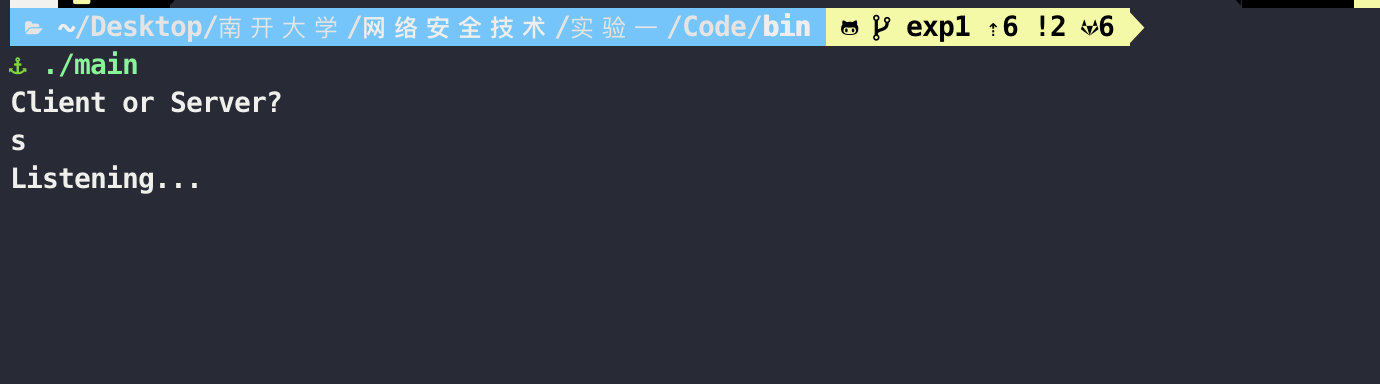
\includegraphics[scale = 0.5]{1}
\end{center}
客户端上线,连接成功
\begin{center}
  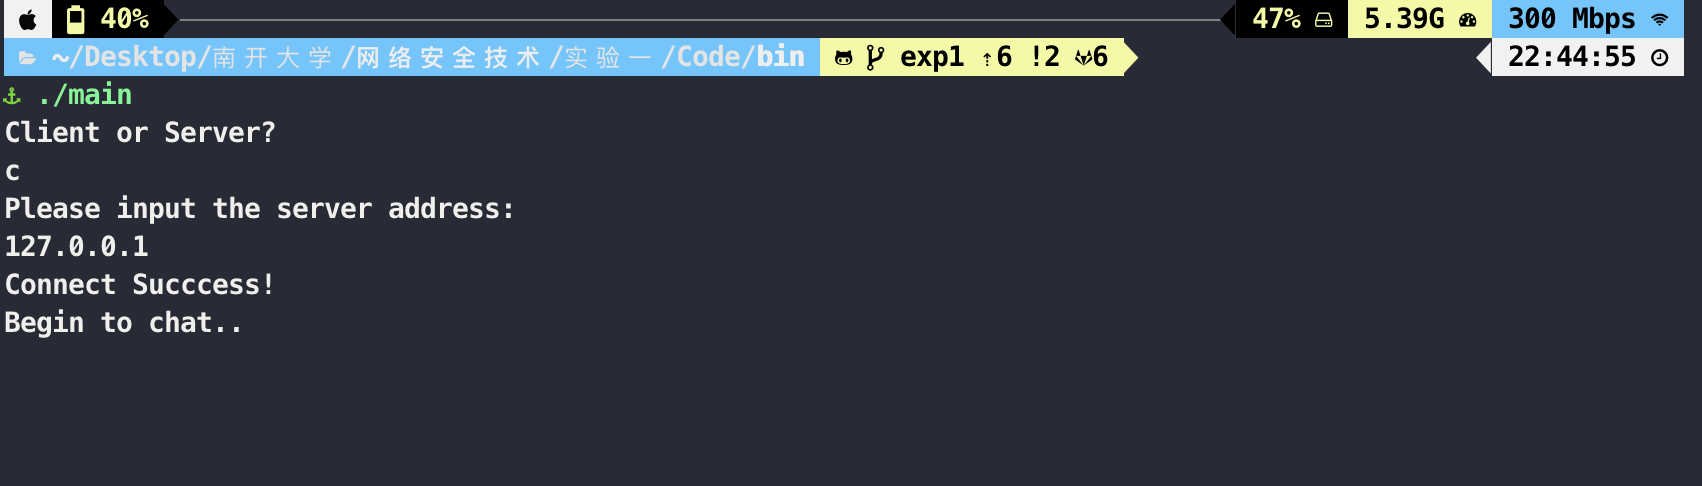
\includegraphics[scale = 0.5]{2}
\end{center}
客户端向服务端发送消息并成功收到
\begin{center}
  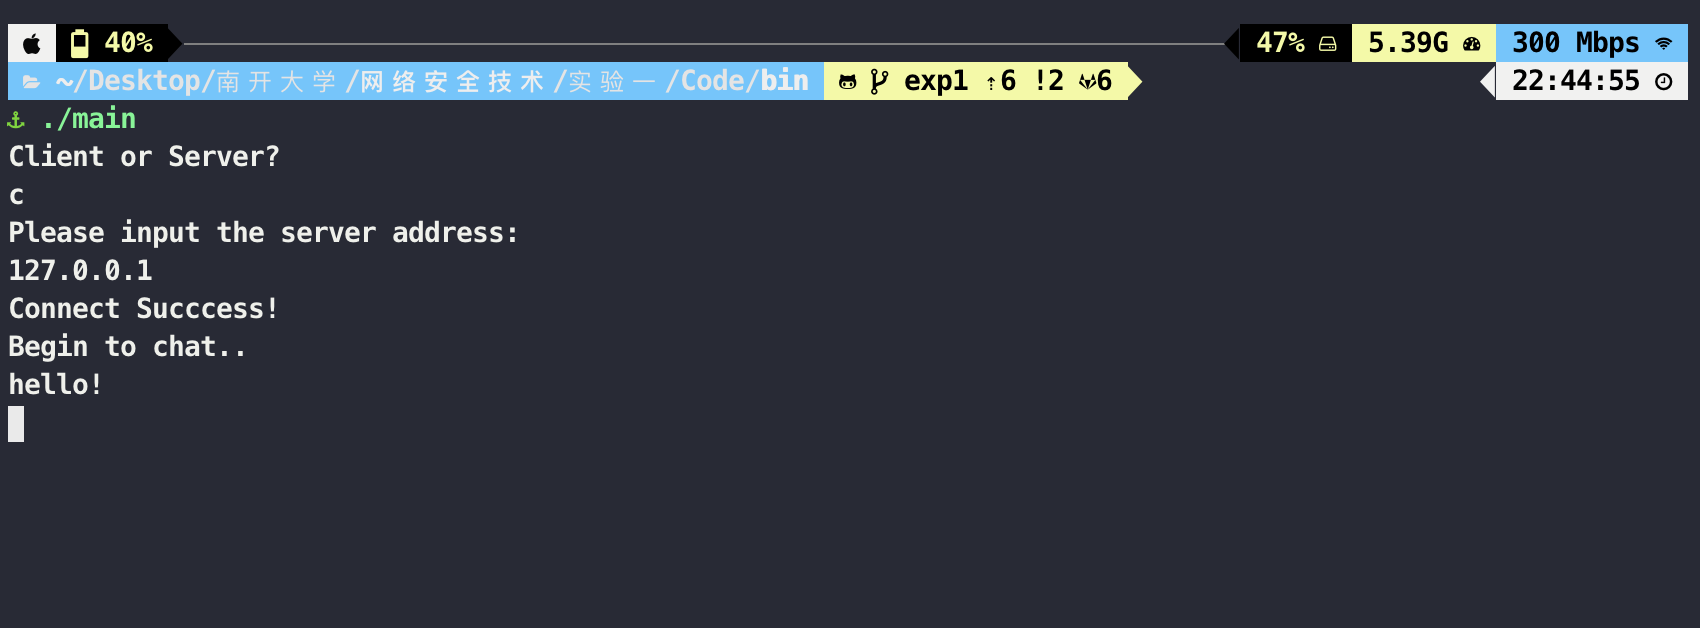
\includegraphics[scale = 0.5]{3}
  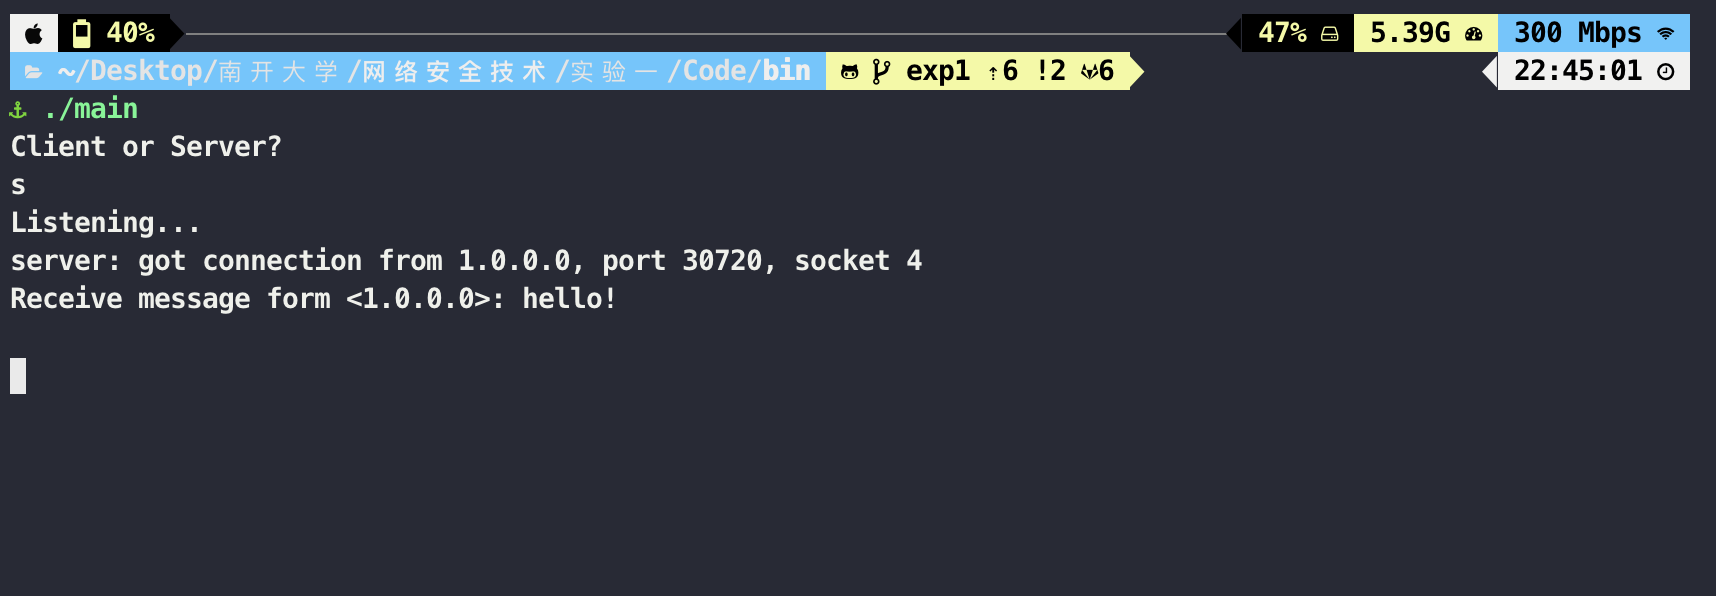
\includegraphics[scale = 0.5]{4}
\end{center}
服务端向客户端发送消息并成功收到
\begin{center}
  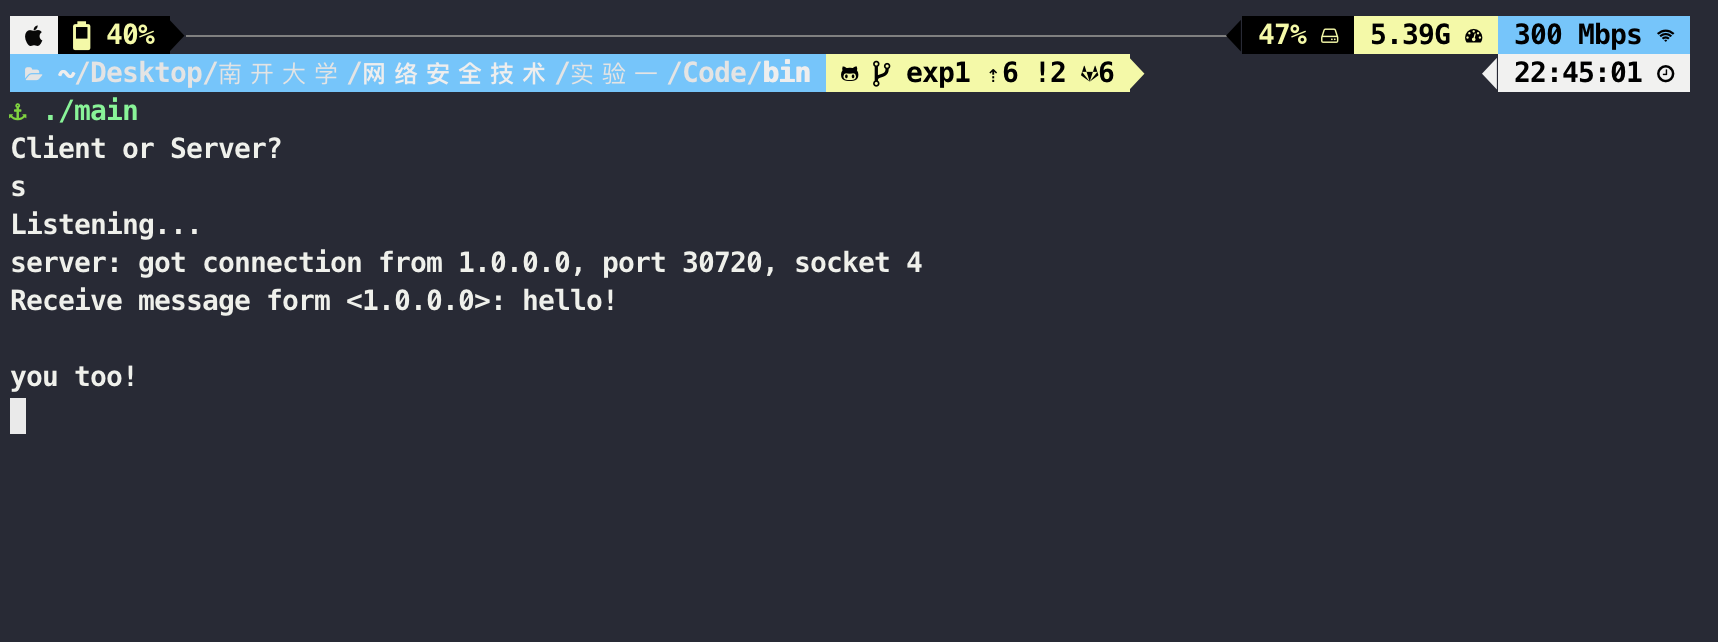
\includegraphics[scale = 0.5]{5}
  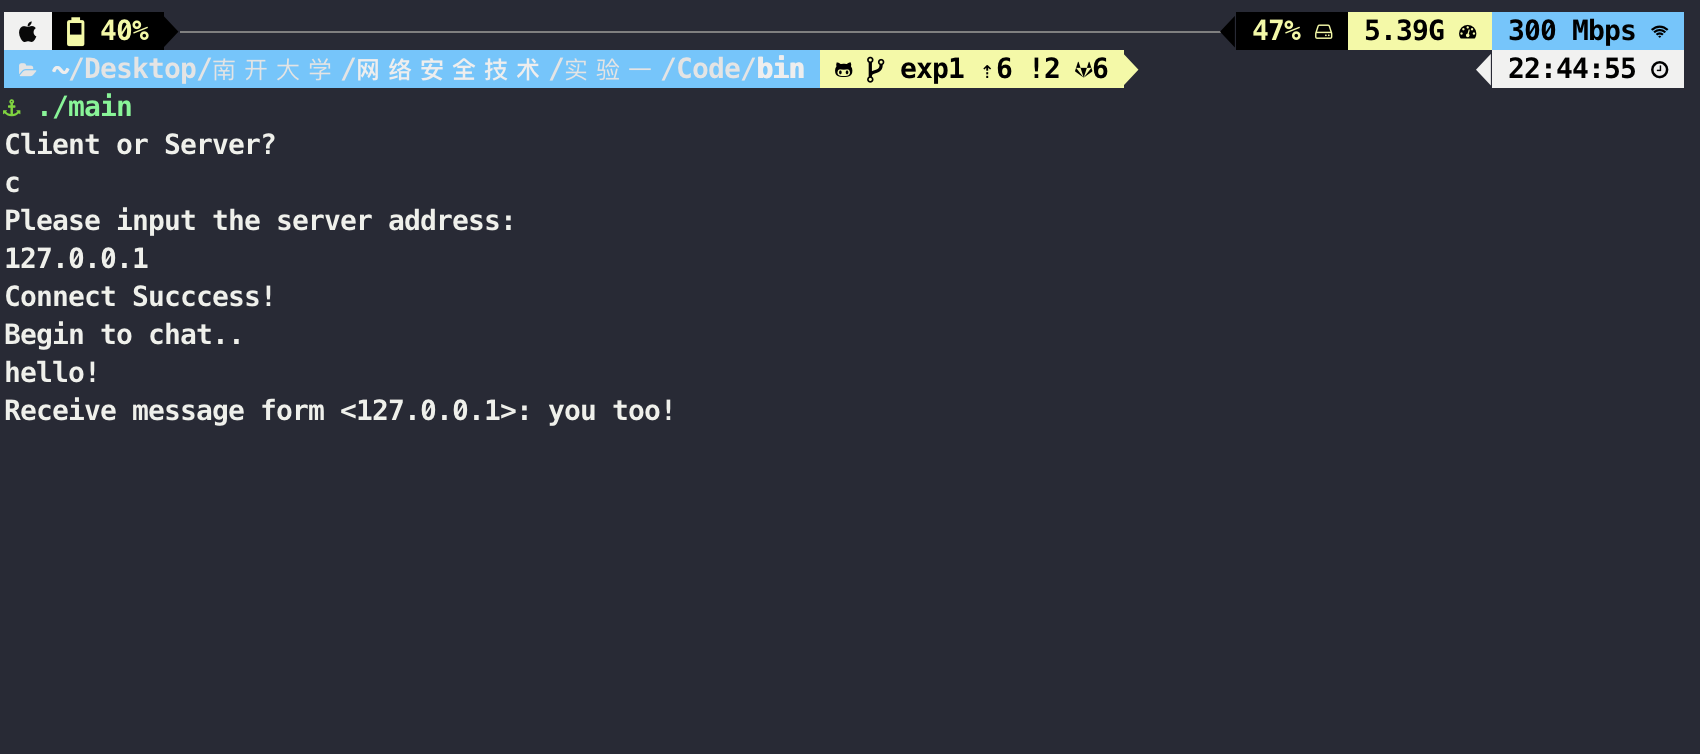
\includegraphics[scale = 0.5]{6}
\end{center}
退出程序
\begin{center}
  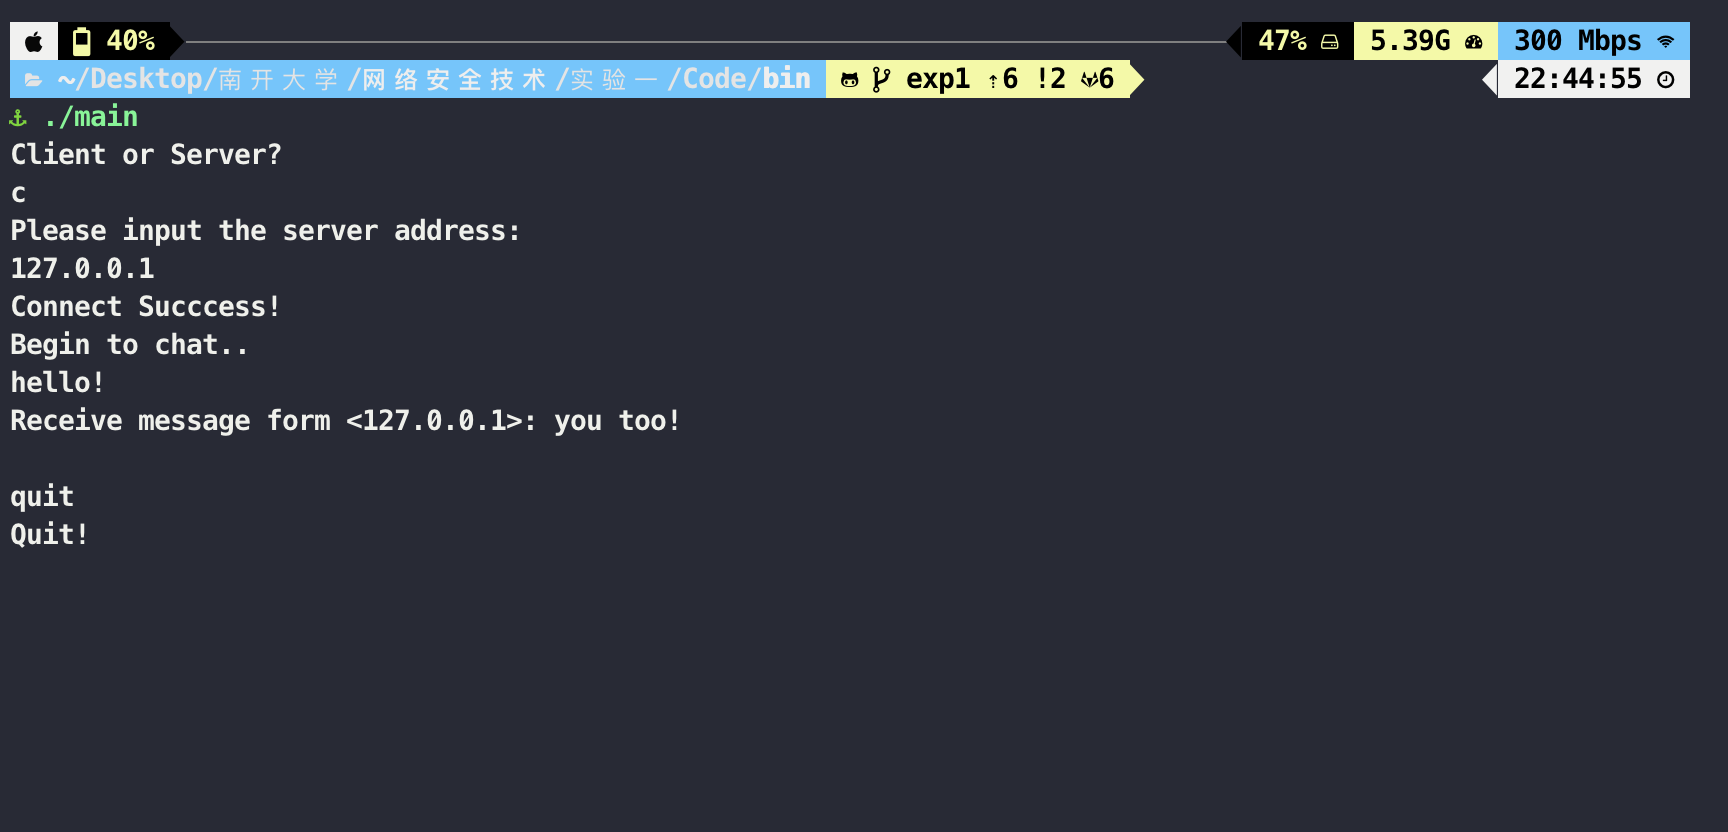
\includegraphics[scale = 0.5]{7}
  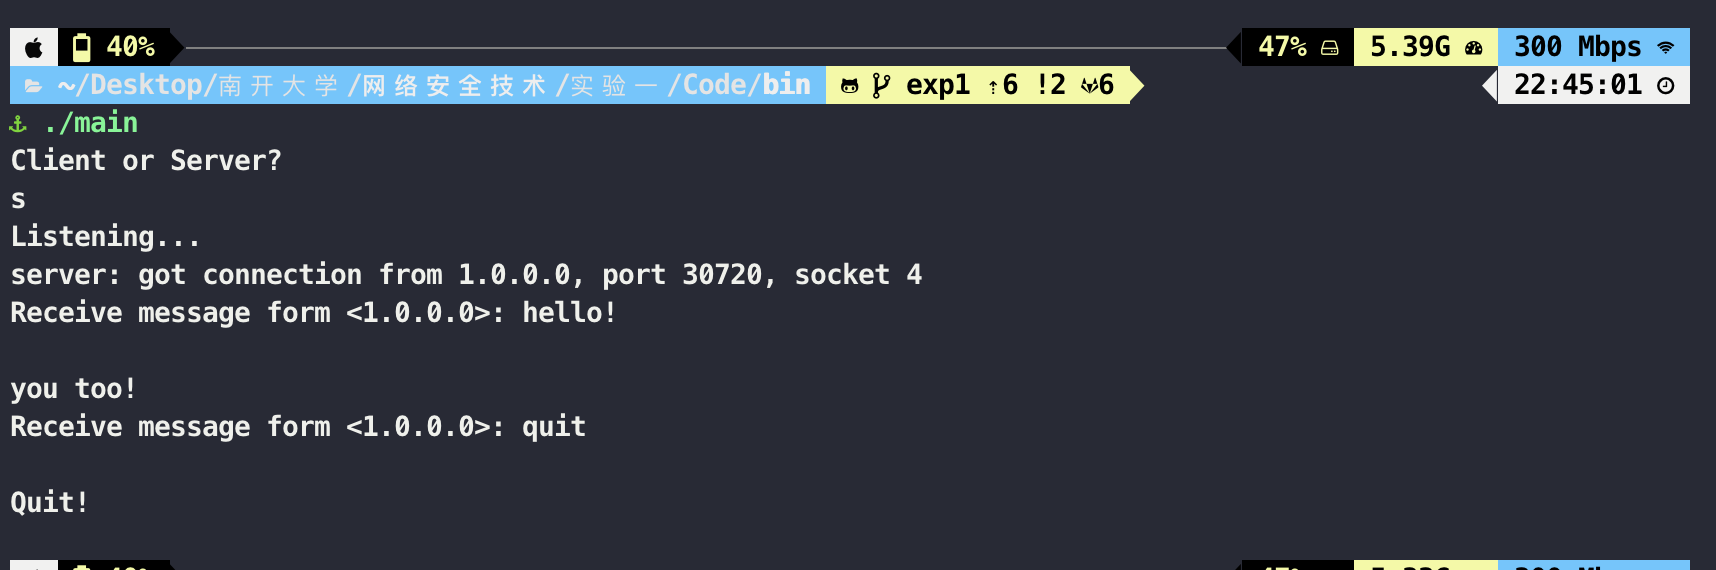
\includegraphics[scale = 0.5]{8}
\end{center}

\section{实验遇到的问题及其解决方法}

\section{实验结论}








\section{概述}
%——————————————————————————————————————
\subsection{第一节}
如图\ref{fig:1}所示
\begin{figure}[H]
    \centering
    
\includegraphics[scale=0.3]{NKU.png}
    \caption{Caption}
    \label{fig:1}
\end{figure}

表
\begin{table}[!htbp]
  \centering
  \begin{tabular}{ccccccccccc}
  \toprule  
  N/n$\backslash$Algo& naive-conv& naive-pool& omp-conv& omp-pool\\
  \midrule
  64/2& 0.0167& 0.01255& 0.04142& 0.03799\\
  64/4& 0.03599&0.0394& 0.0458& 0.0421\\
  \bottomrule
  \end{tabular}
  \caption{性能测试结果(4线程)(单位:ms)}
\end{table}

带单元格表格
\begin{table}[!htbp]
  \centering
  \begin{tabular}{|c|c|c|c|c|c|c|}
  \hline
  \multicolumn{2}{|c|}{ \multirow{2}*{$Cost$} }& \multicolumn{5}{c|}{To}\\
  \cline{3-7}
  \multicolumn{2}{|c|}{}&$A$&$B$&$C$&$D$&$E$\\
  \hline
  \multirow{3}*{From}&$B$&7&0&1&3&8\\
  \cline{2-7}
  &$C$&8&1&0&2&7\\
  \cline{2-7}
  &$D$&8&3&2&0&5\\
  \hline
  \end{tabular}
  \caption{结点C距离向量表(无毒性逆转)}
\end{table}

%——————————————————————————————————————
\subsection{第二节}
伪代码

\begin{breakablealgorithm} 
  \caption{初始化obj文件信息——对应MeshSimplify类中readfile函数,Face类calMatrix函数} 
  \begin{algorithmic}[1] %每行显示行号  
      \Require obj文件,顶点、边、面列表
      \Ensure 是否读取成功
      \Function {calMatrix}{$Face$}  
              \State $normal \gets e1×e2$  
              \State $normal \gets normal/normal.length$
              \State $temp[] \gets {normal.x, normal.y, normal.z, normal· Face.v1}$
              \State $Matrix[i][j]=temp[i] * temp[j]$ 
              \State \Return{$Matrix$}  
      \EndFunction
      \State 根据obj的v和f区分点面信息,读取并加入列表
      \State $scale \gets $记录点坐标中距离原点最远的分量,以便后续OpenGL进行显示
      \State $ori \gets $记录中心点,便于OpenGL显示在中心位置,避免有的obj偏移原点较多
      \State 根据三角面片信息,计算一个面的三条边
      \State 计算每个面的矩阵$\gets calMatrix$
      \State 将每个面的矩阵加到各点,由点维护\\
      \Return True
  \end{algorithmic}  
\end{breakablealgorithm}

代码
\begin{lstlisting}[title=逐列访问平凡算法,frame=trbl,language={C++}]
  void ord()   
  {
      double head,tail,freq,head1,tail1,timess=0; // timers
      init(N);
      QueryPerformanceFrequency((LARGE_INTEGER *)&freq );
      QueryPerformanceCounter((LARGE_INTEGER *)&head);
      for (int i=0; i<NN; i++)
          for (int j=0; j<NN; j++)
              col_sum[i] += (b[j][i]*a[j]);
      QueryPerformanceCounter ((LARGE_INTEGER *)& tail) ;
      cout << "\nordCol" <<(tail-head)*1000.0 / freq<< "ms" << endl;
  }
\end{lstlisting}


%——————————————————————————————————————
\subsection{第三节}

参考文献\cite{adams1995hitchhiker}\cite{shin2016deep}
    
多行公式
\begin{align}
  a+b = a + b \\
  \frac{a+b}{a-b}
\end{align}

行内公式:$\sum^N_{i=1}$

\textbf{超链接}  \href{http://youtube.com/}{YouTube}

带标号枚举
\begin{enumerate}
  \item 1
  \item 2
\end{enumerate}

不带标号枚举
\begin{itemize}
  \item 1
  \item 2
\end{itemize}

\xiaosi{切换字体大小}

%----------------------------------------------------------------
\section{总结}

%----------------------------------------------------------------
\newpage
\bibliographystyle{plain}
\bibliography{references} 
\end{document}
